\documentclass[]{book}
\usepackage{lmodern}
\usepackage{amssymb,amsmath}
\usepackage{ifxetex,ifluatex}
\usepackage{fixltx2e} % provides \textsubscript
\ifnum 0\ifxetex 1\fi\ifluatex 1\fi=0 % if pdftex
  \usepackage[T1]{fontenc}
  \usepackage[utf8]{inputenc}
\else % if luatex or xelatex
  \ifxetex
    \usepackage{mathspec}
  \else
    \usepackage{fontspec}
  \fi
  \defaultfontfeatures{Ligatures=TeX,Scale=MatchLowercase}
\fi
% use upquote if available, for straight quotes in verbatim environments
\IfFileExists{upquote.sty}{\usepackage{upquote}}{}
% use microtype if available
\IfFileExists{microtype.sty}{%
\usepackage{microtype}
\UseMicrotypeSet[protrusion]{basicmath} % disable protrusion for tt fonts
}{}
\usepackage[margin=1in]{geometry}
\usepackage{hyperref}
\hypersetup{unicode=true,
            pdftitle={A Reader on Data Visualization},
            pdfauthor={MSIS 2629 Spring 2018},
            pdfborder={0 0 0},
            breaklinks=true}
\urlstyle{same}  % don't use monospace font for urls
\usepackage{natbib}
\bibliographystyle{apalike}
\usepackage{color}
\usepackage{fancyvrb}
\newcommand{\VerbBar}{|}
\newcommand{\VERB}{\Verb[commandchars=\\\{\}]}
\DefineVerbatimEnvironment{Highlighting}{Verbatim}{commandchars=\\\{\}}
% Add ',fontsize=\small' for more characters per line
\usepackage{framed}
\definecolor{shadecolor}{RGB}{248,248,248}
\newenvironment{Shaded}{\begin{snugshade}}{\end{snugshade}}
\newcommand{\KeywordTok}[1]{\textcolor[rgb]{0.13,0.29,0.53}{\textbf{#1}}}
\newcommand{\DataTypeTok}[1]{\textcolor[rgb]{0.13,0.29,0.53}{#1}}
\newcommand{\DecValTok}[1]{\textcolor[rgb]{0.00,0.00,0.81}{#1}}
\newcommand{\BaseNTok}[1]{\textcolor[rgb]{0.00,0.00,0.81}{#1}}
\newcommand{\FloatTok}[1]{\textcolor[rgb]{0.00,0.00,0.81}{#1}}
\newcommand{\ConstantTok}[1]{\textcolor[rgb]{0.00,0.00,0.00}{#1}}
\newcommand{\CharTok}[1]{\textcolor[rgb]{0.31,0.60,0.02}{#1}}
\newcommand{\SpecialCharTok}[1]{\textcolor[rgb]{0.00,0.00,0.00}{#1}}
\newcommand{\StringTok}[1]{\textcolor[rgb]{0.31,0.60,0.02}{#1}}
\newcommand{\VerbatimStringTok}[1]{\textcolor[rgb]{0.31,0.60,0.02}{#1}}
\newcommand{\SpecialStringTok}[1]{\textcolor[rgb]{0.31,0.60,0.02}{#1}}
\newcommand{\ImportTok}[1]{#1}
\newcommand{\CommentTok}[1]{\textcolor[rgb]{0.56,0.35,0.01}{\textit{#1}}}
\newcommand{\DocumentationTok}[1]{\textcolor[rgb]{0.56,0.35,0.01}{\textbf{\textit{#1}}}}
\newcommand{\AnnotationTok}[1]{\textcolor[rgb]{0.56,0.35,0.01}{\textbf{\textit{#1}}}}
\newcommand{\CommentVarTok}[1]{\textcolor[rgb]{0.56,0.35,0.01}{\textbf{\textit{#1}}}}
\newcommand{\OtherTok}[1]{\textcolor[rgb]{0.56,0.35,0.01}{#1}}
\newcommand{\FunctionTok}[1]{\textcolor[rgb]{0.00,0.00,0.00}{#1}}
\newcommand{\VariableTok}[1]{\textcolor[rgb]{0.00,0.00,0.00}{#1}}
\newcommand{\ControlFlowTok}[1]{\textcolor[rgb]{0.13,0.29,0.53}{\textbf{#1}}}
\newcommand{\OperatorTok}[1]{\textcolor[rgb]{0.81,0.36,0.00}{\textbf{#1}}}
\newcommand{\BuiltInTok}[1]{#1}
\newcommand{\ExtensionTok}[1]{#1}
\newcommand{\PreprocessorTok}[1]{\textcolor[rgb]{0.56,0.35,0.01}{\textit{#1}}}
\newcommand{\AttributeTok}[1]{\textcolor[rgb]{0.77,0.63,0.00}{#1}}
\newcommand{\RegionMarkerTok}[1]{#1}
\newcommand{\InformationTok}[1]{\textcolor[rgb]{0.56,0.35,0.01}{\textbf{\textit{#1}}}}
\newcommand{\WarningTok}[1]{\textcolor[rgb]{0.56,0.35,0.01}{\textbf{\textit{#1}}}}
\newcommand{\AlertTok}[1]{\textcolor[rgb]{0.94,0.16,0.16}{#1}}
\newcommand{\ErrorTok}[1]{\textcolor[rgb]{0.64,0.00,0.00}{\textbf{#1}}}
\newcommand{\NormalTok}[1]{#1}
\usepackage{longtable,booktabs}
\usepackage{graphicx,grffile}
\makeatletter
\def\maxwidth{\ifdim\Gin@nat@width>\linewidth\linewidth\else\Gin@nat@width\fi}
\def\maxheight{\ifdim\Gin@nat@height>\textheight\textheight\else\Gin@nat@height\fi}
\makeatother
% Scale images if necessary, so that they will not overflow the page
% margins by default, and it is still possible to overwrite the defaults
% using explicit options in \includegraphics[width, height, ...]{}
\setkeys{Gin}{width=\maxwidth,height=\maxheight,keepaspectratio}
\IfFileExists{parskip.sty}{%
\usepackage{parskip}
}{% else
\setlength{\parindent}{0pt}
\setlength{\parskip}{6pt plus 2pt minus 1pt}
}
\setlength{\emergencystretch}{3em}  % prevent overfull lines
\providecommand{\tightlist}{%
  \setlength{\itemsep}{0pt}\setlength{\parskip}{0pt}}
\setcounter{secnumdepth}{5}
% Redefines (sub)paragraphs to behave more like sections
\ifx\paragraph\undefined\else
\let\oldparagraph\paragraph
\renewcommand{\paragraph}[1]{\oldparagraph{#1}\mbox{}}
\fi
\ifx\subparagraph\undefined\else
\let\oldsubparagraph\subparagraph
\renewcommand{\subparagraph}[1]{\oldsubparagraph{#1}\mbox{}}
\fi

%%% Use protect on footnotes to avoid problems with footnotes in titles
\let\rmarkdownfootnote\footnote%
\def\footnote{\protect\rmarkdownfootnote}

%%% Change title format to be more compact
\usepackage{titling}

% Create subtitle command for use in maketitle
\newcommand{\subtitle}[1]{
  \posttitle{
    \begin{center}\large#1\end{center}
    }
}

\setlength{\droptitle}{-2em}
  \title{A Reader on Data Visualization}
  \pretitle{\vspace{\droptitle}\centering\huge}
  \posttitle{\par}
  \author{MSIS 2629 Spring 2018}
  \preauthor{\centering\large\emph}
  \postauthor{\par}
  \predate{\centering\large\emph}
  \postdate{\par}
  \date{2018-04-26}

\usepackage{booktabs}
\usepackage{amsthm}
\makeatletter
\def\thm@space@setup{%
  \thm@preskip=8pt plus 2pt minus 4pt
  \thm@postskip=\thm@preskip
}
\makeatother

\usepackage{amsthm}
\newtheorem{theorem}{Theorem}[chapter]
\newtheorem{lemma}{Lemma}[chapter]
\theoremstyle{definition}
\newtheorem{definition}{Definition}[chapter]
\newtheorem{corollary}{Corollary}[chapter]
\newtheorem{proposition}{Proposition}[chapter]
\theoremstyle{definition}
\newtheorem{example}{Example}[chapter]
\theoremstyle{definition}
\newtheorem{exercise}{Exercise}[chapter]
\theoremstyle{remark}
\newtheorem*{remark}{Remark}
\newtheorem*{solution}{Solution}
\begin{document}
\maketitle

{
\setcounter{tocdepth}{1}
\tableofcontents
}
\chapter{Preface}\label{preface}

This is a collaborative writing project as part of the course MSIS 2629
``Data Visualization'' at \href{http://www.scu.edu}{Santa Clara
University}. The purpose of the class reader is to collaboratively
engage with and reflect on data visualizations, to establish a solid
theoretical background, and to collect useful practices and showcases.
More information on the background of this project is available in the
\href{https://mschermann.github.io/msis2629spring2018}{syllabus}.

The following text serves explains how we organize ourselves.

\section{References}\label{references}

\textbf{EVERY} references must be included in the \texttt{book.bib}
file. This file uses the bibtex notation (Learn how to use bibtex
\href{http://www.bibtex.org/Using/}{here}.). Most literature search
engines allow you to export the reference information in Bibtex. For
websites we use the following minimal notation (you may add further
information - usually the more the better is a good strategy):

\begin{verbatim}
@misc{great_viz,
  author = {{A great visualizer}},
  year = {1982},
  title = {A ficticious web page title},
  howpublished = {\url{http://great_viz_org/}},
  note = {Accessed: 2018-04-26}
}
\end{verbatim}

Particularly important is the \texttt{note} field. Websites change
frequently, so links will break. If we do this correctly,
\texttt{{[}@great\_viz{]}} will produce \citep{great_viz}.

\section{Images}\label{images}

Images should not be loaded from external website because the links may
change. Instead download a version of the image and create a reference
that contains the link to the image. For example the following image is
a deceptive visualization (the bars do start at zero).

\begin{figure}
\centering
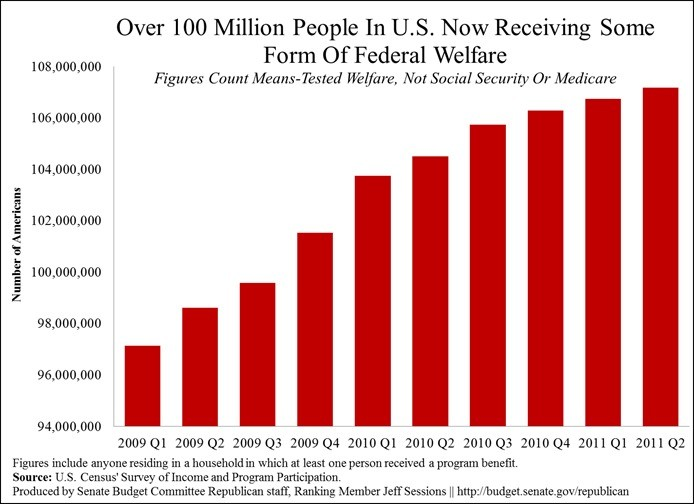
\includegraphics{images/halper_welfare.jpg}
\caption{An Example of a deceptive visualization}
\end{figure}

Source: \citep{halper_2012} referenced in \citep{andale_2014}

The citation for the image looks like this.

\begin{verbatim}
@misc{halper_2012,
  author={Halper, Daniel},
  year={2012},
  title = {Over 100 Million Now Receiving Federal Welfare},
  url={https://www.weeklystandard.com/daniel-halper/over-100-million-now-receiving-federal-welfare},
  note = {Accessed: 2018-04-26}
}
\end{verbatim}

You have probably found this image through a different website that
explains the visualization. For example the following website explains
some problematic aspects of this visualization:

\begin{verbatim}
@misc{andale_2014,
  author={Andalde, Stephanie},
  year={2014},
  title = {Misleading Graphs: Real Life Examples},
  url={http://www.statisticshowto.com/misleading-graphs/},
  note = {Accessed: 2018-04-26}
}
\end{verbatim}

\chapter{Introduction}\label{intro}

\textbf{\#Data Visualization} Data visualization refers to representing
data in a visual context to help people understand the significance of
that data. A way so that information, numbers, and measurements makes
sense is a form of art -- the art of data visualization. Graphs do that
for us.

Plot links: \url{https://datavizcatalogue.com/search.html}

\url{https://infogram.com/page/data-visualization}

You can label chapter and section titles using \texttt{\{\#label\}}
after them, e.g., we can reference Chapter \ref{intro}. If you do not
manually label them, there will be automatic labels anyway, e.g.,
Chapter \ref{methods}.
\url{https://research.tableau.com/user/robert-kosara}
\url{https://twitter.com/eagereyes?ref_src=twsrc\%5Egoogle\%7Ctwcamp\%5Eserp\%7Ctwgr\%5Eauthor}

\url{https://data-visualization.cioreview.com/cxoinsight/what-is-data-visualization-and-why-is-it-important-nid-11806-cid-163.html}

The article , written by Chris Pittenturf, VP-Data \& Analytics, Palace
Sports \& Entertainment, talks about what data visualization is and its
importance to the businesses today. The article begins with a definition
of data visualization in simple terms and goes on to explain how a good
data visualization should be visually engaging to the reader. Chris goes
on to explain the basic criterias that a data visualization should
satisfy to be an effective visualization. These criterias and their
brief meanings are as follows: 1. Informative: The visualization should
be able to convey the information of the data to the reader 2.
Efficient: The visualization should not be ambiguous. 3. Appealing: The
visualization should be captivating and visually pleasing. 4. (Optional)
Interactive and Predictive: The visualizations can contain variables and
filters for the users to interact with the visualizations in order to
predict results of different scenarios.

Chris goes on to give various day-to-day examples where visualization
gives a better understanding of the data. One extremely simple example
used by Chris is that of an energy bill. Chris states that as a
consumer, when we receive an energy bill, we normally look at the graph
in the bill first before proceeding to read the text in the bill. Chris
states that consumers are more likely to analyze and understand the
visualizations before reading further along. The article ends with Chris
emphasizing the importance of data visualizations in our businesses as
well as in our daily lives. According to me, the article gives a simple,
short and crisp understanding of what data visualization is and how it
is relevant to everyone. It shows that data visualization is an aid to
get a better understanding of the complex insights that any business
data provides. Most of the data used by the businesses is highly
unstructured and these businesses can get a better understanding of
their businesses by visualizing their data.

\url{https://www.interaction-design.org/literature/article/information-visualization-a-brief-introduction}
This article is a brief introduction to Information Visualization. It
explains briefly how information visualization helps to make sense of
data, how it helps to find relationships between data and confirm ideas.

About David McCandless's TED talk on data visualization:
\url{https://www.ted.com/talks/david_mccandless_the_beauty_of_data_visualization}

Visuals help us understand concepts that would otherwise be difficult to
contextualize---for example, expenditures or valuations of extremely
large amounts of money are represented in the billion dollar-o-gram by
color-coded, relatively-sized boxes. Furthermore, it allows synthesis of
a breadth of information to be delivered in a small, easily-digestible,
aesthetically pleasing way. Visuals serve as a sort of map for a vast
landscape of information---they direct your eyes to the important places
and details. And the eye, as McCandless notes, is uniquely suited among
our senses to process large amounts of information and detect patterns.

The billion dollar-o-gram is extremely readable and rather pretty, but
it seems a bit dubious to compare the predicted Iraq War cost to the
``mushroomed'' actual cost of Iraq and Afghanistan wars, since its
purpose seems only to conflate two wars for dramatic effect.

Beyond its ability to make information from several different sources
and in large amounts more quickly and easily understood, data
visualization can also reveal smaller interesting patterns---allowing us
to play the ``data detective'' as McCandless calls it. In other words,
as we have already discussed, data visualization can not only be
extremely effective in a declarative manner, but can also be used as an
exploratory tool.

McCandless also postulates that we all have a latent ``design literacy''
that is being developed every day as we are constantly bombarded with
visuals, and that our minds and our eyes are taking in this information
and processing it so that we all have an intuitive sense of design, and
have actually begun to demand a visual aspect to our information. This
is an interesting perspective, since everyone does seem to have a sense
of visual aspects---space, color, etc., but of course the time-honored
adage tells us that beauty is in the eye of the beholder. So while it
might be whimsical to claim that we are all designers, there is still,
of course, great value in learning formal principles of design.\\
Figures and tables with captions will be placed in \texttt{figure} and
\texttt{table} environments, respectively.

\begin{Shaded}
\begin{Highlighting}[]
\KeywordTok{par}\NormalTok{(}\DataTypeTok{mar =} \KeywordTok{c}\NormalTok{(}\DecValTok{4}\NormalTok{, }\DecValTok{4}\NormalTok{, .}\DecValTok{1}\NormalTok{, .}\DecValTok{1}\NormalTok{))}
\KeywordTok{plot}\NormalTok{(pressure, }\DataTypeTok{type =} \StringTok{'b'}\NormalTok{, }\DataTypeTok{pch =} \DecValTok{19}\NormalTok{)}
\end{Highlighting}
\end{Shaded}

\begin{figure}

{\centering 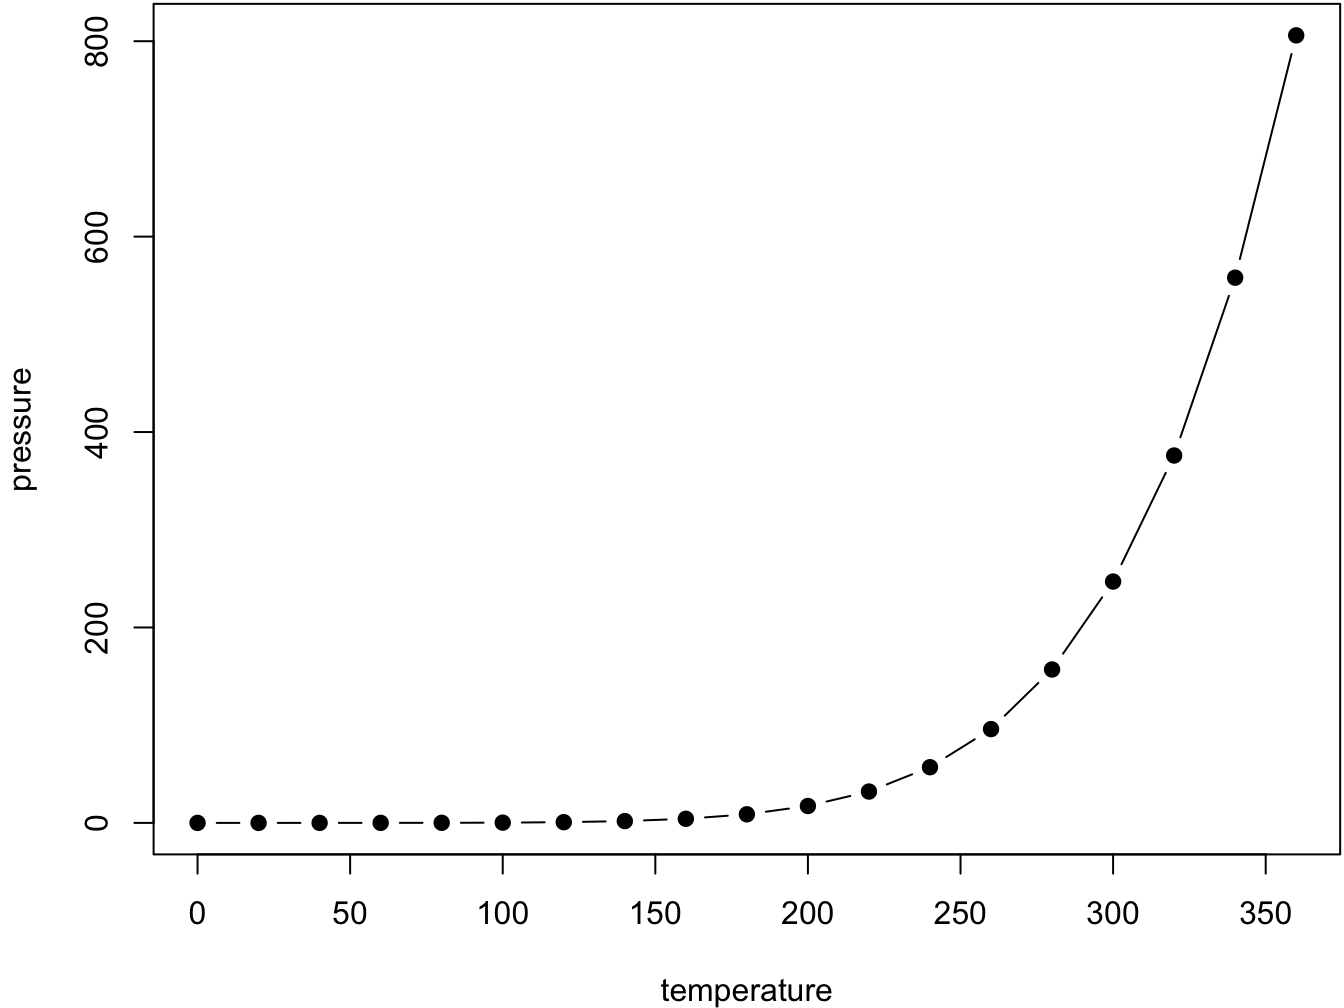
\includegraphics[width=0.8\linewidth]{Data_Viz_Reader_files/figure-latex/nice-fig-1} 

}

\caption{Here is a nice figure!}\label{fig:nice-fig}
\end{figure}

Reference a figure by its code chunk label with the \texttt{fig:}
prefix, e.g., see Figure \ref{fig:nice-fig}. Similarly, you can
reference tables generated from \texttt{knitr::kable()}, e.g., see Table
\ref{tab:nice-tab}.

\begin{Shaded}
\begin{Highlighting}[]
\NormalTok{knitr}\OperatorTok{::}\KeywordTok{kable}\NormalTok{(}
  \KeywordTok{head}\NormalTok{(iris, }\DecValTok{20}\NormalTok{), }\DataTypeTok{caption =} \StringTok{'Here is a nice table!'}\NormalTok{,}
  \DataTypeTok{booktabs =} \OtherTok{TRUE}
\NormalTok{)}
\end{Highlighting}
\end{Shaded}

\begin{table}

\caption{\label{tab:nice-tab}Here is a nice table!}
\centering
\begin{tabular}[t]{rrrrl}
\toprule
Sepal.Length & Sepal.Width & Petal.Length & Petal.Width & Species\\
\midrule
5.1 & 3.5 & 1.4 & 0.2 & setosa\\
4.9 & 3.0 & 1.4 & 0.2 & setosa\\
4.7 & 3.2 & 1.3 & 0.2 & setosa\\
4.6 & 3.1 & 1.5 & 0.2 & setosa\\
5.0 & 3.6 & 1.4 & 0.2 & setosa\\
\addlinespace
5.4 & 3.9 & 1.7 & 0.4 & setosa\\
4.6 & 3.4 & 1.4 & 0.3 & setosa\\
5.0 & 3.4 & 1.5 & 0.2 & setosa\\
4.4 & 2.9 & 1.4 & 0.2 & setosa\\
4.9 & 3.1 & 1.5 & 0.1 & setosa\\
\addlinespace
5.4 & 3.7 & 1.5 & 0.2 & setosa\\
4.8 & 3.4 & 1.6 & 0.2 & setosa\\
4.8 & 3.0 & 1.4 & 0.1 & setosa\\
4.3 & 3.0 & 1.1 & 0.1 & setosa\\
5.8 & 4.0 & 1.2 & 0.2 & setosa\\
\addlinespace
5.7 & 4.4 & 1.5 & 0.4 & setosa\\
5.4 & 3.9 & 1.3 & 0.4 & setosa\\
5.1 & 3.5 & 1.4 & 0.3 & setosa\\
5.7 & 3.8 & 1.7 & 0.3 & setosa\\
5.1 & 3.8 & 1.5 & 0.3 & setosa\\
\bottomrule
\end{tabular}
\end{table}

You can write citations, too. For example, we are using the
\textbf{bookdown} package \citep{R-bookdown} in this sample book, which
was built on top of R Markdown and \textbf{knitr} \citep{xie2015}.

\chapter{Fundamentals}\label{fundamentals}

Due to the rise of big data analytics, there has been an increased need
for data visualization tools to help understand the data. Besides
Tableau, there are several other software tools one can use for data
visualization like Sisense, Plotly, FusionCharts, Highcharts,
Datawrapper, and Qlikview. This article is from forbes and has a brief,
clear introduction about these 7 powerful software options for data
visualization. This could be helpful for future reference because for
different purposes I may need to use different tools. Each option has
its advantages and disadvantages and this article helps highlight them.

Tableau is the most popular of the group and has many users. It is
simple to use, making it easy to learn and can handle large datasets.
Tableau can handle big data thanks to integration with database handling
applications such as MySQL, Hadoop, and Amazon AWS.

Qlikview is the main competitor to Tableau and is also quite popular.
Qlikview is customizable and has a wide range of features which can be a
double-edged sword. These features take more time to learn and get
acquianted with. However, once one gets past the learning curve, they
have a powerful tool at their disposal.

The distinctive aspect of FusionCharts is that graphics do not have to
be created from scratch. Users can start with a template and insert
their own data from their project.

Highcharts proudly claims to be used by 72\% of the 100 biggest
companies in the world. It is a simple tool that does not require
specialized training and quickly generates the desired output. Unlike
some tools, Highcharts focuses on cross-browser support, allowing for
greater access and use.

Datawrapper is making a name for itself in the media industry. It has a
simple user interface making it easy to generate charts and embed into
reports.

Plotly can create more sophisticated visuals thanks to integration with
programming languages such as Python and R. The danger is creating
something more complicated than necessary. The whole point of data
visualization is to quickly and clearly convey information.

Sisense can bring together multiple sources of data for easier access.
It can even work with large datasets. Sisense makes it easy to share
finished products across departments, ensuring everyone can get the
information they need.

\url{https://www.forbes.com/sites/bernardmarr/2017/07/20/the-7-best-data-visualization-tools-in-2017/\#3a12b8ea6c30}

\begin{itemize}
\tightlist
\item
  Theoretical background of data visualization
\end{itemize}

\textbf{Practitioners Guide to Best Practices in Data Visualization}

\textbf{Reference} Jeffrey D. Camm, Michael J. Fry, Jeffrey Shaffer
(2017) A Practitioner's Guide to Best Practices in Data
Visualization.Interfaces 47(6):473-488.
\url{https://doi.org/10.1287/inte.2017.0916}

These are the best practices of data visualization. Anticipate in
advance what kind of questions the viewers will ask and then focus your
visualization with respect to those questions.

Brain processes stimuli from our environment to process what is
important in 2 ways -- unconscious (System 1 represents uncontrolled
functions such as facial expressions, reactions) and conscious (System 2
-- represents controlled function such as solving math problems). Data
Visualization leverage attributes of System -1 which has can have quick
and correct impact in a most efficient manner. The three best practices
of data visualization are as follows: -

** 1. Design and layout matter \textbf{ The design and layout should
facilitate ease of understanding to convey your message to the viewer. }
2. Avoid Clutter \textbf{ Keep it simple. To implement this always keep
into account the data-ink ratio -- the ratio of ink required to convey
the intended meaning to the total amount of ink used in the table or
chart should be as close to 1 as possible. That means, avoid ink which
do not add any information. } 3. Use color purposely and effectively **
Use of color may be prettier and attractive but can be distractive too.
Thus, color should be used only if it assists in conveying your message.
The above three principles are illustrated with the help of scenarios
and examples which helps to comprehend the topic in more meaningful and
practical way in the article. It also gives various advantages of using
the above principles.And the above best practices could be applied to
all the 3 types of analytics: descriptive, predictive and prescriptive.

\begin{itemize}
\item
  Theoretical background of data visualization

  \begin{itemize}
  \tightlist
  \item
    \url{https://www.klipfolio.com/blog/intuitive-dashboard-design}
    Three rules to follow in order to develop intuitive dashboards:
  \end{itemize}

  \begin{enumerate}
  \def\labelenumi{\arabic{enumi}.}
  \tightlist
  \item
    the dashboard should read left to right
  \item
    group related information together
  \item
    find relationships between seemingly unrelated areas and display
    visuals together to show the relationship.
  \end{enumerate}

  Often a designer can become too concerned with coming up with a visual
  that is too intricate and overly complicated. A dashboard should be
  appealing but also easy to understand. Following these rules will lead
  to effective presentation of the data.

  Because we read from top to bottom and left to right, a reader's eyes
  will naturally look in the upper left of a page. The content should
  therefore flow like words in a book. It is important to note that the
  information at the top of the page does not always have to be the most
  important. Annual data is usually more important to a business but
  daily or weekly data could be used more often for day to day work.
  This should be kept in mind when designing a dashboard as dashboards
  are often used as a quick convenient way to look up data.

  Grouping related data together is an intuitive way to help the flow of
  the visual. It does not make sense for a user to have to search in
  different areas to find the information they need.

  Grouping unrelated data seems contradictory to the second rule, but
  the important thing is to tell a story not previously observed. Data
  analytics is all about finding stories the data is trying to tell.
  Once they are discovered, the stories need to be presented in an
  effective manner. Grouping unrelated data together makes it easier to
  see how they change together.
\item
  Theoretical background of data visualization

  \begin{enumerate}
  \def\labelenumi{\arabic{enumi}.}
  \item
    Fundamental Components of Design

    Artists use balance, emphasis, movement, pattern, repetition,
    proportion, rhythm, variety, and unity as the design foundation of
    any work. If you want to take your data visualization from an
    everyday dashboard to a compelling data story, incorporate the 9
    principles of design from graphic designer Melissa Anderson's
    article:
    \url{https://www.idashboards.com/blog/2017/07/26/data-visualization-and-the-9-fundamental-design-principles/}

    Balance doesn't mean that each side of the visualization needs
    perfect symmetry, but it is important to have the elements of the
    dashboard/visualiaztion distributed evenly. And it important to
    remember the non-data elements, such as a logo, title, caption,
    etc., that can affect the balance of the display.

    Another closely related component to balance is variety which could
    seem counter to balance, but when done correctly, variety can help
    increase the recall of information. However if overdone, too much
    variety can feel cluttered and blur together the images and data in
    the mind of the viewer.

    Arguably the most critical of the components is proportion.
    Proportion can be subtle but it can go a long way to enhancing a
    viewer's experience and understanding of the data. The danger of
    proportion though is that it can be easy to deceive people
    subconsciously. Naturally images will have a greater impact on how
    our brains perceive the dashboard or visualization. For example,
    someone can change the scale of a graph or images to inflate their
    results and even if they write the numbers next to it, the shortcut
    many people will take is to interpret the data based on the image.
    This is why it is important we take care to accurately reflect
    proportion in our data visualization and remain critical of how
    others use proportion in their visualization.

    Emphasis was the component that I most related to when reading
    through the nine principles of design in this article. From prior
    experience with art through photography I understand it is key to be
    concious of what I am drawing the viewers attention to in my art.
    When thinking about the art design of data visualization it is also
    very important to remain keen on the main point of your story and
    how the entire visualization is either drawing the viewer to that
    point of emphasis or how they are being distracted or drawn
    elsewhere.
  \end{enumerate}
\item
  Theoretical background of data visualization

  \textbf{A Brief History of Data Visualization }

  \textbf{Reference}

  Michael Friendly,2006,A Brief History of Data Visualization,York
  University.\url{http://www.datavis.ca/papers/hbook.pdf}

  The only new thing in the world is the history you don't know. ---
  Harry S Truman

  This paper provides an overview of the intellectual history of data
  visualization from medieval to modern times, describing and
  illustrating some significant advances along the way.
\end{itemize}

\begin{enumerate}
\def\labelenumi{\arabic{enumi}.}
\item
  Data Visualization: modern product?

  It is common to think of statistical graphics and data visualization
  as relatively modern developments in statistics. In fact, the graphic
  representation of quantitative information has deep roots.These roots
  reach into the histories of the earliest map-making and visual
  depiction, and later into thematic cartography, statistics and
  statistical graphics, medicine, and other fields.

  Developments in technologies (printing, reproduction) mathematical
  theory and practice, and empirical observation and\\
  recording, enabled the wider use of graphics and new advances in form
  and content.

  \begin{enumerate}
  \def\labelenumii{\arabic{enumii}.}
  \setcounter{enumii}{1}
  \tightlist
  \item
    Milestones Tour
  \end{enumerate}

  2.1 Pre-17th Century: Early maps and diagrams

\begin{verbatim}
  The earliest seeds of visualization arose in geometric diagrams, in tables of the positions of stars and other
  celestial bodies, and in the making of maps to aid in navigation and exploration. 
\end{verbatim}

  2.2 1600-1699: Measurement and theory

\begin{verbatim}
  Among the most important problems of the 17th century were those concerned with physical measurement— of time,
  distance,and space— for astronomy, surveying, map making, navigation and territorial expansion. This century also
  saw great new growth in theory and the dawnof practical application.
\end{verbatim}

  2.3 1700-1799: New graphic forms

\begin{verbatim}
  With some rudiments of statistical theory, data of interest and importance, and the idea of graphic representation
  at least somewhat established, the 18th century witnessed the expansion of these aspects to new domains and new
  graphic forms. 
\end{verbatim}

  2.4 1800-1850: Beginnings of modern graphics

\begin{verbatim}
  With the fertilization provided by the previous innovations of design and technique, the first half of the 19th
  century witnessed explosive growth in statistical graphics and thematic mapping, at a rate which would not be
  equalled until modern times.
\end{verbatim}

  2.5 1850--1900: The Golden Age of statistical graphics

\begin{verbatim}
  By the mid-1800s, all the conditions for the rapid growth of visualization had been established— a “perfect storm”
  for data graphics. Official state statistical offices were established throughout Europe, in recognition of the
  growing importance of numerical information for social planning,industrialization, commerce, and transportation. 

   2.5.1 Escaping flatland
   2.5.2 Graphical innovations
   2.5.3 Galton’s contributions
   2.5.4 Statistical Atlases
\end{verbatim}

  2.6 1900-1950: The modern dark ages

\begin{verbatim}
  If the late 1800s were the “golden age” of statistical graphics and thematic cartography, the early 1900s can be
  called the “modern dark ages” of visualization. There were few graphical innovations, and, by the mid-1930s, the
  enthusiasm for visualization which characterized the late 1800s had been supplanted by the rise of quantification
  and formal, often statistical, models in the social sciences.
\end{verbatim}

  2.7 1950--1975: Re-birth of data visualization

\begin{verbatim}
  Still under the influence of the formal and numerical zeitgeist from the mid-1930s on, data visualization began to
  rise from dormancy in the mid 1960s. 
\end{verbatim}

  2.8 1975--present: High-D, interactive and dynamic data visualization

\begin{verbatim}
  During the last quarter of the 20th century data visualization has blossomed into a mature, vibrant and multi
  disciplinary research area, as may be seen in this Handbook, and software tools for a wide range of visualization
  methods and data types are available for every desktop computer.
\end{verbatim}
\end{enumerate}

\begin{itemize}
\tightlist
\item
  Contemporary research results
\item
  Contemporary research results reference---fundamentals--example-USDATA
\end{itemize}

\textbf{Contemporary research results}

\begin{itemize}
\item
  Next Steps for Data Visualization Research
\item
  references:
  \url{https://medium.com/@uwdata/next-steps-for-data-visualization-research-3ef5e1a5e349}

  With the development, studies and new tools applied in data
  visualization, more people understand it matters. But given its youth
  and interdisciplinary nature, research methods and training in the
  field of data visualization are still developing. So, we asked
  ourselves: what steps might help accelerate the development of the
  field? Based on a group brainstorm and discussion, this article shares
  some of the proposals of ongoing discussion and experiment with new
  approaches:
\end{itemize}

\begin{enumerate}
\def\labelenumi{\arabic{enumi}.}
\tightlist
\item
  Adapting the Publication and Review Process
\end{enumerate}

\begin{itemize}
\tightlist
\item
  As the article states, ``both `good' and `bad' reviews could serve as
  valuable guides'', so providing reviewer guidelines could be helpful
  for fledgling practitioners in the field.
\end{itemize}

\begin{enumerate}
\def\labelenumi{\arabic{enumi}.}
\setcounter{enumi}{1}
\tightlist
\item
  Promoting Discussion and Accretion
\end{enumerate}

\begin{itemize}
\tightlist
\item
  Discussion of research papers actively occurs at conferences, on
  social media, and within research groups. Much of this discussion is
  either ephemeral or non-public. So ongoing discussion might explicitly
  transition to the online forum.
\end{itemize}

\begin{enumerate}
\def\labelenumi{\arabic{enumi}.}
\setcounter{enumi}{2}
\tightlist
\item
  Research Methods Training
\end{enumerate}

\begin{itemize}
\item
  Developing a core curriculum for data visualization research might
  help both cases, guiding students and instructors alike. For example,
  recognizing that empirical methods were critical to multiple areas of
  computer science, Stanford CS faculty organized a new course on
  Designing Computer Science
  Experiments(\url{http://sing.stanford.edu/cs303-sp11/}). Also, online
  resources could be reinforced with a catalog of learning resources,
  ranging from tutorials and self-guided study to online courses. Useful
  examples include Jake Wobbrock's Practical Statistics for HCI and
  Pierre Dragicevic's resources for reforming statistical practice.
\item
  Contemporary research results
\end{itemize}

Pick the Right Chart Type!

Data divusalization is combining the art and science. As for the art, we
can say there are no correct answers for doing the visualization. There
are many ways to present the data. However, how to making sense of
facts, numbers and measurement for better understanding is still have a
logical path to follow.

To determine which kind of chart is hard for those people new to data
visulization. Most people learn it by refering some other people's work
without understanding the logic behind. So they don't have the theory in
their mind to make the judgement. Here , I will introduce some guidance
to choose the charts.

When we about to choose the type of chart, we need to answer some
questions. - How many features would you like to show in a chart? - how
many data points do you want to display for each variable? - Will you
display time serious data or among items or groups.

After answered this question, you shoul able to get a better imagenation
of your ideal graph. The simple guidance for using different type of
chart is line charts for tracking trends over time, bar charts to
compare quantities, scatter plots for joint variation of two data items,
bubble charts showing joint variation of three data items, and pie
charts to compare parts of a whole.

Let's review the most commonly used chart types and expalin what
circumstance should better use typical chart and the pros and conts of
each type of chart. Before introduce differnt types of charts, you can
use the following website to familiar with different types of charts.
\href{https://datavizcatalogue.com/}{The Data Visualisation Catalogue}

\#\# Type 1 Column Charts. This should be the most popular chart type.
This chart is good to do comparison between different values when
specific values are important. TBD

Still have hard time to choose? There are many resources on line can
help you do the decision. For example, Dr.~Andre Abela create a chart
selection diagram that is helpful to pick the right chart depends on the
data type. The link of website is
\url{http://extremepresentation.typepad.com/blog/2015/01/announcing-the-slide-chooser.html}

Reference: Data Visualization -- How to Pick the Right Chart Type? , By
Jānis Gulbis
\url{https://eazybi.com/blog/data_visualization_and_chart_types/}

Data Visualization Best Practices by melindasantos \textbar{} Sep 19,
2017 \url{http://paristech.com/blog/data-visualization-best-practices/}

\url{http://paristech.com/blog/data-visualization-best-practices/}
\url{http://extremepresentation.typepad.com/blog/2015/01/announcing-the-slide-chooser.html}

Misleading graphs: Misleading graphs or distorted graphs, are graphs
created which skews the data, intentionally or unintentionally,
resulting in a representation of incorrect conclusions. There are some
ways in which distorted graphs can be created: 1. Improper scaling of y
axis: This is one of the classic misleading graphs. Instead of scale
starting from zero or a baseline, y axis is scaled conveniently to
highlight the differences among bins. 2. Improper labelling of graphs:
Lack of labels make the graph hard to interpret for the reader and lead
to wrong conclusions. 3. Paired graphs on different scale: It is not a
fair comparison if two elements are plotted side-by-side, on a different
scale and compared. This makes one graph look better than the other,
even when it is not. 4. Dual axis with different scales: If we are
plotting two elements on the same graph with different scales, even if
the axes are properly labeled, it is assumed that both axes are on the
same scale. 5. Incomplete data: Short-term graphs are made to manipulate
the trend, which will not be seen otherwise. Time-series data are cut
intentionally to just show a trend within a particular period to create
a more favorable visual impression.

Please find the references below.
\url{http://hypsypops.com/axes-evil-lie-graphs/}
\url{http://www.statisticshowto.com/misleading-graphs/}

\begin{itemize}
\tightlist
\item
  Theoretical background of data visualization
\end{itemize}

\textbf{Definions of Date Deception and Graphic Integrity}

\textbf{Reference} (1) Pandey, A. V., Rall, K., Satterthwaite, M. L.,
Nov, O., \& Bertini, E. (2015). How deceptive are deceptive
visualizations? An empirical analysis of common distortion techniques.
In CHI 2015 - Proceedings of the 33rd Annual CHI Conference on Human
Factors in Computing Systems: Crossings (Vol. 2015-April,
pp.~1469-1478). Association for Computing Machinery. DOI:
10.1145/2702123.2702608 (2) Tufte, E. R., and Graves-Morris, P. The
visual display of quantitative information, vol.~2. Graphics press
Cheshire, CT, 1983.

Data visualization becomes more and more pupular to communicate and
support arguments nowdays. There are lots of great resources online to
create and design amazing data products, in the same time, there are
some poorly-designed misleading deceptive data visualizations.

So what does \textbf{data deception} mean? Data deception, defined by
School of Law at the New York University, as ``a graphical depiction of
information, designed with or without an intent to deceive, that may
create a belief about the message and/or its components, which varies
from the actual message.''

In reality, decades ago, Edward Tufte already introduced the concept of
graphical intergrity in his book and presented six principles of graphic
integrity. Here are the principles from book:

\begin{enumerate}
\def\labelenumi{\arabic{enumi}.}
\item
  The representation of numbers, as physically measured on the surface
  of the graphic itself, should be directly proportional to the
  numerical quantities measured.
\item
  Clear, detailed, and thorough labeling should be used to defeat
  graphical distortion and ambiguity. Write out explanations of the data
  on the graphic itself. Label important events in the data.
\item
  Show data variation, not design variation.
\item
  In time-series displays of money, deflated and standardized units of
  monetary measurement are nearly always better than nominal units.
\item
  The number of information-carrying (variable) dimensions depicted
  should not exceed the number of dimensions in the data.
\end{enumerate}

6.Graphics must not quote data out of context.

\chapter{Case Studies}\label{case-studies}

\begin{itemize}
\tightlist
\item
  Description and replication of great examples of data visualization
  \#\#\# Description and replication of great examples of data
  visualization
\end{itemize}

reference:\url{http://blog.visme.co/best-information-graphics-2016/\#e030mFiF7wCpk7Ld.99}

\begin{enumerate}
\def\labelenumi{\arabic{enumi}.}
\tightlist
\item
  Connecting the Dots Behind the Election
\end{enumerate}

\url{https://www.nytimes.com/interactive/2015/05/17/us/elections/2016-presidential-campaigns-staff-connections-clinton-bush-cruz-paul-rubio-walker.html?_r=1}

This article by the New York Times lists several different candidates
and creates compelling visuals that link their campaigns to previous
ones.

Each visual contains several different-sized dots that represent a
specific campaign, administration, or other governmental organization
related to the candidate's current campaign, which are then connected by
arrows.

Hovering over a specific dot highlights the connections between the
groups. The visual is a great way to put what would otherwise be a long
slog through years of information into an easily accessible, easily
viewable format so that voters can figure out where the candidates'
experiences lie.

\begin{enumerate}
\def\labelenumi{\arabic{enumi}.}
\setcounter{enumi}{1}
\tightlist
\item
  Spies in the Skies
\end{enumerate}

\url{https://www.buzzfeed.com/peteraldhous/spies-in-the-skies?utm_term}=.so1GQ6ZGDo\#.ec8kL3WkZe

The map is filled with red and blue lines (representing FBI and DHS
aircraft, respectively) which illustrate the flight paths of the planes.
When planes circle an area more than once, the circles become darker.
The circles change in accordance to day and time, and individual cities
can be typed into a search bar to see the flight patterns over them.

The visualization, rather creatively, almost looks like a hand-drawn
map. While presenting a normally uncomfortable topic, this allows
individuals to check things for themselves, hopefully providing some
peace of mind.

\begin{enumerate}
\def\labelenumi{\arabic{enumi}.}
\setcounter{enumi}{2}
\tightlist
\item
  Green Honey
\end{enumerate}

\url{http://muyueh.com/greenhoney/?es_p=1228877}

The visualization spans a webpage. As you scroll down, the text changes,
as do many colored dots that move over the white background. The dots
are used to represent not only each colors' hue, but the numbers that
fall into each category---for example, what colors are the most popular
``base'' colors for English and Chinese.

The continuous flow of this visualization helps really bring it
together, allowing users to scroll through the information at their own
pace, but also creating a seamless, creative work.

\begin{enumerate}
\def\labelenumi{\arabic{enumi}.}
\setcounter{enumi}{3}
\tightlist
\item
  How People Like You Spend Their Time
\end{enumerate}

\url{http://flowingdata.com/2016/12/06/how-people-like-you-spend-their-time/}

The visual lists several categories along one side of a graph---such as
``personal care'' and ``work''---with a line illustrating the amount of
time the average person in a certain demographic spends on each subject.
Entering different statistics at the top---such as changing gender or
age---causes the lines to shift to feature that demographic.

The simplicity of this visualization really helps the information get
across and avoids bogging down the statistics. Sometimes, less is more.

\begin{enumerate}
\def\labelenumi{\arabic{enumi}.}
\setcounter{enumi}{4}
\tightlist
\item
  Is it Better to Rent or Buy?
\end{enumerate}

\url{https://www.nytimes.com/interactive/2014/upshot/buy-rent-calculator.html?_r=0}

The calculator includes several sloping charts. Each chart includes a
factor that'll affect how much you'll have to pay, such as the
individual cost of your home and your mortgage rates. A movable scale
along the bottom of each chart allows you to enter different data,
changing the ``cost of rent per month'' on the side. If you can find a
similar house to rent for that much per month or less, it's more cost
effective to just rent the home.

This visualization is incredibly thorough and a useful tool for
homeowners of any age and status.

\section{Deceptive data graphs
examples}\label{deceptive-data-graphs-examples}

references: **Misleading Graphs: Real Life Examples
\url{http://www.statisticshowto.com/misleading-graphs/**}

Misleading graphs are sometimes deliberately misleading and sometimes
it's just a case of people not understanding the data behind the graph
they create. But some real life misleading graphs go above and beyond
the classic types. Some are intended to mislead, others are intended to
shock. The ``classic'' types of misleading graphs include cases where:

\begin{itemize}
\tightlist
\item
  \textbf{The Missing Baseline.}
\end{itemize}

For example, the Vertical scale is too big or too small, or skips
numbers, or doesn't start at zero, like the graph below:

You might be thinking that the graph on the right shows The Times makes
double the sales of The Daily Telegraph. But take a closer look at the
scale and you'll see although The Times does make more sales, it's only
beating the competition by about 10\%.

\begin{itemize}
\tightlist
\item
  \textbf{The graph isn't labeled properly.}
\end{itemize}

Graghs can have the correct figures, but still can mislead you.

This one used a BIG HEADLINE makes you think that 5.3\% of children get
spinal cord injuries which is a pretty scary statistic for parents. But
the real figure is about .0000003\% (based on 2000 injuries per year out
of a population of around 74,000,000).

And for the figure 1 used in this article: Misleading Graphs: Displaying
a Change in One Variable Using Area or Volume
\url{https://www.forbes.com/sites/naomirobbins/2012/02/28/misleading-graphs-displaying-a-change-in-one-variable-using-area-or-volume/\#696674551781},
the label for the smaller triangle in this graph says \$26.4 while the
label for the larger triangle says \$114.6. \$114.6 is 4.34 times
\$26.4. It certainly looks to me as if more than 4.34 smaller triangles
will fit in the larger triangle. It is the altitudes of the triangles
that are proportional to the numbers in the labels.

\begin{itemize}
\tightlist
\item
  \textbf{Data is left out.}
\end{itemize}

Only include part of the data like the following graph which using
temperatures of the first half of the year to prove it was rising
dramatically.

For more examples of misleading graphs or deceptive graphs you can read
the following articles for more inspirations:

\begin{itemize}
\tightlist
\item
  bar charts without zero \& evenly spaced tick marks for uneven
  intervals:
  \url{https://www.forbes.com/sites/naomirobbins/2011/11/17/whats-wrong-with-this-graph/\#502ab1a42a33}
\item
  graphs not drawn to scale:
  \url{https://www.forbes.com/sites/naomirobbins/2012/02/16/misleading-graphs-figures-not-drawn-to-scale/\#351dcf9c15ef}
\end{itemize}

\begin{enumerate}
\def\labelenumi{\arabic{enumi}.}
\setcounter{enumi}{5}
\tightlist
\item
  What's really warming the world?
\end{enumerate}

\url{https://www.bloomberg.com/graphics/2015-whats-warming-the-world/}

In this case study, it first claimed the background story and the
analytical questions clearly. Then it analyzed each different factors
separately using both verbal explanations and dynamic graphics to
compare with the observed temperature movements, and then grouped
related factors into Natural factors category or Human factors category.
After that, it combined all the dynamic graphics into one and made the
results more straightforward in terms of comparisons. In the end, the
authors also provided more detailed methodology explanations with
dataset sources to support the results shown above.

Overall, this case study is straightforward, easy to understand but also
with enough information shown on each graphics.

\chapter{Patterns}\label{patterns}

\begin{itemize}
\tightlist
\item
  Reusable solutions to everyday data visualization questions
\item
  Applied by multiple members of the course
\end{itemize}

\section{Why pie chart is bad: a comparison with bar
chart}\label{why-pie-chart-is-bad-a-comparison-with-bar-chart}

Using pie chart is usually considered as a bad idea when it comes to
data visualization. But why? Here, we explore some cons of using pie
chart to convey information and compare its effectiveness to bar chart
\citep{hickey-pie-worst} \citep{henry-defense-pie} \citep{quach-penny}.

\begin{enumerate}
\def\labelenumi{\arabic{enumi}.}
\item
  Some information may look nearly identical in pie chart. But if the
  data is presented with bar charts, the story is different.
\item
  It is difficult to compare the slices of a circle to figure out the
  distinctions in size between each pie slice, especially when there are
  a lot of categories.
\item
  Pie chart is easy to be manipulated (e.g.~using a 3D pie chart).
\item
  Pie chart may be useful when comparing 2 different categories with
  different amounts of information. Specifically, it does a better job
  to distinguish two parts with a 25:75 split or one that is not 50:50
  as people are sensitive to a right angle or a dividing line that is
  not straight. But this could be simply done by showing two numbers!
\end{enumerate}

\section{Chose the right baseline in data
visualization}\label{chose-the-right-baseline-in-data-visualization}

Baseline is very important to data visualization. If baseline is
different, the meanning will change a lot. Now here is a case study to
show the importance of baseline and how to use it in different ways.

Here I use the same method for a new dataset to .

\begin{Shaded}
\begin{Highlighting}[]
\CommentTok{# Load the data.}
\CommentTok{#setwd("/Users/boxiao/Desktop")}
\NormalTok{data<-}\KeywordTok{read.csv}\NormalTok{(}\StringTok{"galaxy_sales.csv"}\NormalTok{,}\DataTypeTok{header =} \OtherTok{TRUE}\NormalTok{)}
\NormalTok{data <-}\StringTok{ }\KeywordTok{rbind}\NormalTok{(data[}\DecValTok{1}\OperatorTok{:}\DecValTok{19}\NormalTok{,],}\KeywordTok{c}\NormalTok{(}\StringTok{"Q4 '14"}\NormalTok{,}\DecValTok{80}\NormalTok{),data[}\DecValTok{20}\OperatorTok{:}\DecValTok{22}\NormalTok{,],}\KeywordTok{c}\NormalTok{(}\StringTok{"da"}\NormalTok{, }\DecValTok{83}\NormalTok{))}
\NormalTok{data}\OperatorTok{$}\NormalTok{year <-}\StringTok{ }\KeywordTok{rep}\NormalTok{(}\KeywordTok{c}\NormalTok{(}\DecValTok{2010}\NormalTok{,}\DecValTok{2011}\NormalTok{,}\DecValTok{2012}\NormalTok{,}\DecValTok{2013}\NormalTok{,}\DecValTok{2014}\NormalTok{,}\DecValTok{2015}\NormalTok{),}\DataTypeTok{each =} \DecValTok{4}\NormalTok{)}
\NormalTok{data}\OperatorTok{$}\NormalTok{qua <-}\StringTok{ }\KeywordTok{seq}\NormalTok{(}\DecValTok{1}\OperatorTok{:}\DecValTok{24}\NormalTok{)}
\NormalTok{data}\OperatorTok{$}\NormalTok{Quarter <-}\OtherTok{NULL}
\end{Highlighting}
\end{Shaded}

\begin{enumerate}
\def\labelenumi{\arabic{enumi}.}
\tightlist
\item
  Regular quaterly sales. We can see sales decreased a lot around 2014.
  \textbf{The baseline here is historical sales.}
\end{enumerate}

\begin{Shaded}
\begin{Highlighting}[]
\CommentTok{# Regular time series for sales}
\KeywordTok{par}\NormalTok{(}\DataTypeTok{cex.axis=}\FloatTok{0.7}\NormalTok{)}
\NormalTok{data.ts <-}\StringTok{ }\KeywordTok{ts}\NormalTok{(data}\OperatorTok{$}\NormalTok{sales, }\DataTypeTok{start=}\KeywordTok{c}\NormalTok{(}\DecValTok{2010}\NormalTok{, }\DecValTok{1}\NormalTok{), }\DataTypeTok{frequency=}\DecValTok{4}\NormalTok{)}
\KeywordTok{plot}\NormalTok{(data.ts, }\DataTypeTok{xlab=}\StringTok{""}\NormalTok{, }\DataTypeTok{ylab=}\StringTok{""}\NormalTok{, }\DataTypeTok{main=}\StringTok{"sales per quater"}\NormalTok{, }\DataTypeTok{las=}\DecValTok{1}\NormalTok{, }\DataTypeTok{bty=}\StringTok{"n"}\NormalTok{)}
\end{Highlighting}
\end{Shaded}

\begin{enumerate}
\def\labelenumi{\arabic{enumi}.}
\setcounter{enumi}{1}
\tightlist
\item
  Quaterly and yearly change sales. \textbf{The baseline here is zero
  and look at the percentage changes.}
\end{enumerate}

\begin{Shaded}
\begin{Highlighting}[]
 \CommentTok{# Quaterly change}
\NormalTok{curr <-}\StringTok{ }\KeywordTok{as.numeric}\NormalTok{(data}\OperatorTok{$}\NormalTok{sales[}\OperatorTok{-}\DecValTok{1}\NormalTok{])}
\NormalTok{prev <-}\StringTok{ }\KeywordTok{as.numeric}\NormalTok{(data}\OperatorTok{$}\NormalTok{sales[}\DecValTok{1}\OperatorTok{:}\NormalTok{(}\KeywordTok{length}\NormalTok{(data}\OperatorTok{$}\NormalTok{sales)}\OperatorTok{-}\DecValTok{1}\NormalTok{)])}
\NormalTok{quaChange <-}\StringTok{ }\DecValTok{100} \OperatorTok{*}\StringTok{ }\KeywordTok{round}\NormalTok{( (curr}\OperatorTok{-}\NormalTok{prev) }\OperatorTok{/}\StringTok{ }\NormalTok{prev, }\DecValTok{2}\NormalTok{ )}
\NormalTok{barCols <-}\StringTok{ }\KeywordTok{sapply}\NormalTok{(quaChange, }
    \ControlFlowTok{function}\NormalTok{(x) \{ }
        \ControlFlowTok{if}\NormalTok{ (x }\OperatorTok{<}\StringTok{ }\DecValTok{0}\NormalTok{) \{}
            \KeywordTok{return}\NormalTok{(}\StringTok{"#2cbd25"}\NormalTok{)}
\NormalTok{        \} }\ControlFlowTok{else}\NormalTok{ \{}
            \KeywordTok{return}\NormalTok{(}\StringTok{"gray"}\NormalTok{)}
\NormalTok{        \}}
\NormalTok{    \})}
\CommentTok{#monChange.ts <- ts(monChange, start=c(1976, 2), frequency=12)}
\KeywordTok{barplot}\NormalTok{(quaChange, }\DataTypeTok{border=}\OtherTok{NA}\NormalTok{, }\DataTypeTok{space=}\DecValTok{0}\NormalTok{, }\DataTypeTok{las=}\DecValTok{1}\NormalTok{, }\DataTypeTok{col=}\NormalTok{barCols, }\DataTypeTok{main=}\StringTok{"% change, quaterly"}\NormalTok{)}
\end{Highlighting}
\end{Shaded}

\begin{Shaded}
\begin{Highlighting}[]
\CommentTok{# Year-over-year change}
\NormalTok{curr <-}\StringTok{ }\KeywordTok{as.numeric}\NormalTok{(data}\OperatorTok{$}\NormalTok{sales[}\OperatorTok{-}\NormalTok{(}\DecValTok{1}\OperatorTok{:}\DecValTok{4}\NormalTok{)])}
\NormalTok{prev <-}\StringTok{ }\KeywordTok{as.numeric}\NormalTok{(data}\OperatorTok{$}\NormalTok{sales[}\DecValTok{1}\OperatorTok{:}\NormalTok{(}\KeywordTok{length}\NormalTok{(data}\OperatorTok{$}\NormalTok{sales)}\OperatorTok{-}\DecValTok{4}\NormalTok{)])}
\NormalTok{annChange <-}\StringTok{ }\DecValTok{100} \OperatorTok{*}\StringTok{ }\KeywordTok{round}\NormalTok{( (curr}\OperatorTok{-}\NormalTok{prev) }\OperatorTok{/}\StringTok{ }\NormalTok{prev, }\DecValTok{2}\NormalTok{ )}
\NormalTok{barCols <-}\StringTok{ }\KeywordTok{sapply}\NormalTok{(annChange, }
    \ControlFlowTok{function}\NormalTok{(x) \{ }
        \ControlFlowTok{if}\NormalTok{ (x }\OperatorTok{<}\StringTok{ }\DecValTok{0}\NormalTok{) \{}
            \KeywordTok{return}\NormalTok{(}\StringTok{"#2cbd25"}\NormalTok{)}
\NormalTok{        \} }\ControlFlowTok{else}\NormalTok{ \{}
            \KeywordTok{return}\NormalTok{(}\StringTok{"gray"}\NormalTok{)}
\NormalTok{        \}}
\NormalTok{    \})}
\KeywordTok{barplot}\NormalTok{(annChange, }\DataTypeTok{border=}\OtherTok{NA}\NormalTok{, }\DataTypeTok{space=}\DecValTok{0}\NormalTok{, }\DataTypeTok{las=}\DecValTok{1}\NormalTok{, }\DataTypeTok{col=}\NormalTok{barCols, }\DataTypeTok{main=}\StringTok{"% change, annual"}\NormalTok{)}
\end{Highlighting}
\end{Shaded}

From this plot, it is very clear that the magnitude of drops in sales
for some quaters.

\begin{enumerate}
\def\labelenumi{\arabic{enumi}.}
\setcounter{enumi}{2}
\tightlist
\item
  The sales difference compare to now. \textbf{The baseline here is the
  current sales.}
\end{enumerate}

\begin{Shaded}
\begin{Highlighting}[]
\CommentTok{# Relative to current 2015}
\NormalTok{curr <-}\StringTok{ }\KeywordTok{as.numeric}\NormalTok{(data}\OperatorTok{$}\NormalTok{sales[}\KeywordTok{length}\NormalTok{(data}\OperatorTok{$}\NormalTok{sales)])}
\NormalTok{salesDiff <-}\StringTok{ }\KeywordTok{as.numeric}\NormalTok{(data}\OperatorTok{$}\NormalTok{sales) }\OperatorTok{-}\StringTok{ }\NormalTok{curr}
\NormalTok{barCols.diff <-}\StringTok{ }\KeywordTok{sapply}\NormalTok{(salesDiff,}
    \ControlFlowTok{function}\NormalTok{(x) \{}
        \ControlFlowTok{if}\NormalTok{ (x }\OperatorTok{<}\StringTok{ }\DecValTok{0}\NormalTok{) \{}
            \KeywordTok{return}\NormalTok{(}\StringTok{"gray"}\NormalTok{)}
\NormalTok{        \} }\ControlFlowTok{else}\NormalTok{ \{}
            \KeywordTok{return}\NormalTok{(}\StringTok{"black"}\NormalTok{)}
\NormalTok{        \}}
\NormalTok{    \}}
\NormalTok{)}
\KeywordTok{barplot}\NormalTok{(salesDiff, }\DataTypeTok{border=}\OtherTok{NA}\NormalTok{, }\DataTypeTok{space=}\DecValTok{0}\NormalTok{, }\DataTypeTok{las=}\DecValTok{1}\NormalTok{, }\DataTypeTok{col=}\NormalTok{barCols.diff, }\DataTypeTok{main=}\StringTok{"Sales difference from last quater 2015"}\NormalTok{)}
\end{Highlighting}
\end{Shaded}

\begin{enumerate}
\def\labelenumi{\arabic{enumi}.}
\setcounter{enumi}{3}
\tightlist
\item
  Sales difference compared to the first quater. ** The baseline here is
  the first quater sales.**
\end{enumerate}

\begin{Shaded}
\begin{Highlighting}[]
\CommentTok{# Relative to first quater}
\NormalTok{ori <-}\StringTok{ }\KeywordTok{as.numeric}\NormalTok{(data}\OperatorTok{$}\NormalTok{sales[}\DecValTok{1}\NormalTok{])}
\NormalTok{salesDiff <-}\StringTok{ }\KeywordTok{as.numeric}\NormalTok{(data}\OperatorTok{$}\NormalTok{sales) }\OperatorTok{-}\StringTok{ }\NormalTok{ori}
\NormalTok{barCols.diff <-}\StringTok{ }\KeywordTok{sapply}\NormalTok{(salesDiff,}
    \ControlFlowTok{function}\NormalTok{(x) \{}
        \ControlFlowTok{if}\NormalTok{ (x }\OperatorTok{<}\StringTok{ }\DecValTok{0}\NormalTok{) \{}
            \KeywordTok{return}\NormalTok{(}\StringTok{"gray"}\NormalTok{)}
\NormalTok{        \} }\ControlFlowTok{else}\NormalTok{ \{}
            \KeywordTok{return}\NormalTok{(}\StringTok{"black"}\NormalTok{)}
\NormalTok{        \}}
\NormalTok{    \}}
\NormalTok{)}
\KeywordTok{barplot}\NormalTok{(salesDiff, }\DataTypeTok{border=}\OtherTok{NA}\NormalTok{, }\DataTypeTok{space=}\DecValTok{0}\NormalTok{, }\DataTypeTok{las=}\DecValTok{1}\NormalTok{, }\DataTypeTok{col=}\NormalTok{barCols.diff, }\DataTypeTok{main=}\StringTok{"Sales difference from first quater 2010"}\NormalTok{)}
\end{Highlighting}
\end{Shaded}

\begin{enumerate}
\def\labelenumi{\arabic{enumi}.}
\setcounter{enumi}{4}
\tightlist
\item
  The difference between quater sales and mean. ** The baseline is mean
  now.**
\end{enumerate}

\begin{Shaded}
\begin{Highlighting}[]
\CommentTok{# difference from the mean}
\NormalTok{mean <-}\StringTok{ }\KeywordTok{mean}\NormalTok{(}\KeywordTok{as.numeric}\NormalTok{(data}\OperatorTok{$}\NormalTok{sales))}
\NormalTok{salesDiff <-}\StringTok{ }\KeywordTok{as.numeric}\NormalTok{(data}\OperatorTok{$}\NormalTok{sales) }\OperatorTok{-}\StringTok{ }\NormalTok{mean}
\NormalTok{barCols.diff <-}\StringTok{ }\KeywordTok{sapply}\NormalTok{(salesDiff,}
    \ControlFlowTok{function}\NormalTok{(x) \{}
        \ControlFlowTok{if}\NormalTok{ (x }\OperatorTok{<}\StringTok{ }\DecValTok{0}\NormalTok{) \{}
            \KeywordTok{return}\NormalTok{(}\StringTok{"gray"}\NormalTok{)}
\NormalTok{        \} }\ControlFlowTok{else}\NormalTok{ \{}
            \KeywordTok{return}\NormalTok{(}\StringTok{"black"}\NormalTok{)}
\NormalTok{        \}}
\NormalTok{    \}}
\NormalTok{)}
\KeywordTok{barplot}\NormalTok{(salesDiff, }\DataTypeTok{border=}\OtherTok{NA}\NormalTok{, }\DataTypeTok{space=}\DecValTok{0}\NormalTok{, }\DataTypeTok{las=}\DecValTok{1}\NormalTok{, }\DataTypeTok{col=}\NormalTok{barCols.diff, }\DataTypeTok{main=}\StringTok{"Sales difference from mean"}\NormalTok{)}
\end{Highlighting}
\end{Shaded}

So before we start to plot, we should decide the baseline we want to
use. Different baseline will lead to totally different graphs.

Reference: \url{https://flowingdata.com/2013/11/26/the-baseline/}

\chapter{Ethics}\label{ethics}

\begin{itemize}
\tightlist
\item
  Implications of (good and bad) data visualization

  \begin{itemize}
  \tightlist
  \item
    The role of data visualization in politics, society, and business
  \end{itemize}
\end{itemize}

Tableau: Viz of the Day

Tableau has a gallery called Viz of the Day
(\url{https://public.tableau.com/en-us/s/gallery} ) that displays great
data visualization examples created by Tableau. It is cool to see how
people are using all kinds of data to create informative yet fun data
visuals. Data being used is also attached so we can try to mimic what
other people did as well.

One interesting example I found is Describe Artists with Emoji
(\url{https://public.tableau.com/en-us/s/gallery/what-emoji-say-about-music?gallery=featured}).
Using the data from Spotify, the author listed the 10 most distinctive
emoji used in the playlists related to popular artists. The table being
used in this visual is very straight forward to link artist to the
emojis and is very easy to compare among artists. When you hover over
the emoji, further information is presented.

\textbf{1. Data visualization in political and social sciences} -
(Reference:
\url{https://github.com/mschermann/data_viz_reader/files/1933699/Zinovyev_Data_Visualization.pdf})

The basic objective of data visualization is to provide an efficient
graphical display for summarizing and reasoning about quantitative
information. And during the last decades, political science has
accumulated a large corpus of various kinds of data, which makes it
gradually become a more quantitative scientific field and requires using
quantitative information in the analysis and reasoning.

Data visualization plays several important roles in it: 1) helps create
informative illustrations of the data, recapitulating large amount of
quantitative information on a diagram; 2) helps formulate new or
supporting existing hypotheses from quantitative data; 3) guides a
statistical analysis of data and checks its validity.

Some useful visualization methods are: 1) \emph{Statistical graphics and
infographics}; 2) \emph{Geographical information systems (GIS)}; 3)
\emph{Graph visualization or network maps}; 4) \emph{Data cartography}.

\textbf{Misrepresentation through Data Visualization} - (Reference:
\url{https://venngage.com/blog/misleading-graphs/})

While the ideal purpose of data visualization is to improve others'
understanding of the data presented, visualization can also be used to
mislead. Some of the main methods of doing so are omitting baselines,
axis manipulation, omitting data, and going against graphing convention.

Omitting baselines is used to imply a greater difference between two
categories, such as in poll results comparing political parties. Axis
manipulation by increasing the highest value on the y-axis affects the
visibility of a slope, making data with an otherwise visible trend
appear flat. Omitting selected data points or narrowing the window of a
graph is used to hide an overall trend, such as a graph of a stock only
showing a current trend and hiding previous bubbles. Graphs can also be
designed to subvert convention so that at first glance the graph is
conveying the opposite message, for example, by using the reader's
associations of colors and temperature to create a graph where hot is
blue and cold is red.

\textbf{A basis for why we should pursue ethical data visualization}
Reference: Cairo, Alberto. ``Ethical Infographics: In data
visualization, journalism meets engineering.'' The IRE Journal, Spring
2014.
\url{https://www.scribd.com/document/230474170/Ethical-Info-Graphics-In-data-visualization-journalism-meets-engineering}
Cairo, Alberto. The Functional Art weblog. 19 June 2016.
\url{http://www.thefunctionalart.com/2014/06/infographics-data-and-visualization.html}

Alberto Cairo addresses into the ethical `why' of data visualization in
this article, while still grounding the discussion in straightforward
analysis of what to do and what not to do. He emphasizes that the
effectiveness of the communicative display is as important as the
information itself. This makes intuitive sense because useful
information is rendered utterly useless if no one can understand it.

Cairo sees data visualization as a harmonization of journalism and
engineering. From these two disciplines, he takes the journalist ethos
of truth-telling and honesty and combines this with an engineering focus
on efficacy and efficiency. The result is a data visualization that
contains accurate and relevant information which is clearly and
concisely conveyed. Cairo describes himself as a ``rule utilitarian''
and uses this to explain why it is ethical or, in his words, ``morally
right,'' to create graphics in this way. Here, it very useful to review
his blogpost introducing the article.

Essentially, the goal is to create the most good while doing the least
harm. As such, conveying truthful and honest relevant information
increases a persons understanding. Increased understanding and knowledge
positively correlates with personal well-being.

So, the information presented must be accurate and relevant. Cairo
briefly addresses guidelines for this which are applicable in all
information gathering fields: beware of selection bias when choosing
preexisting datasets, validate the data, and include important context.
False or irrelevant information doesn't improve anyone's decision-making
capacity, so it cannot enhance well-being.

Even if the information is both accurate and relevant, moral engineering
pitfalls may remain. To avoid the unethical trap of inscrutable (or
misleading) graphics, Cairo exhorts us to take an evidenced based
approach when possible. The purpose of the graphic dictates the form it
takes; aesthetic preferences should never override clarity.

Again, since the ethical purpose is to improve well-being through
understanding, a graphic which is confusing or misleading is unethical,
regardless of intent, since it actually creates misunderstanding for the
audience. While it can be a bit jarring to think of an poorly designed
graphic as ``morally wrong'', it is important to think of the unintended
consequences of visuals which have a powerful impact on their viewers.

\chapter{Conclusion}\label{conclusion}

Reflection, Key Learnings, Outlook

\chapter*{References}\label{references-1}
\addcontentsline{toc}{chapter}{References}

\textbf{1. 3 Expert Data Visualization Tips for Grabbing Readers'
Attention}

URL:
\url{https://towardsdatascience.com/3-expert-data-visualization-tips-for-grabbing-readers-attention-206d8c4621bf}

\emph{Summary}: This article found on Medium explores three important
aspects to focus on when creating a data visualization. The importance
of each aspect is explained along with helpful questions to ask and to
help you evaluate your visualization to ensure it caters to your
audience. Although it primarily focuses on the appearance of visuals, it
also discusses the psychology of the reader as they're looking at a data
visual, which offers a unique and useful perspective.

Here is an outline of each of the 3 aspects: 1. Know what you really
want to say. We want to share patterns, trends, anomalies, etc. with
others through data visuals but we must find the right things to
represent.

\begin{enumerate}
\def\labelenumi{\arabic{enumi}.}
\setcounter{enumi}{1}
\item
  Design. Visuals should be kept as simple as possible without leaving
  out key points. This makes sense because then the audience can focus
  on what's really important.
\item
  Labeling. This section of the article shows a nice comparison of
  before and after removing labels from a chart, and the `after' chart
  looks much cleaner and easier to interpret.
\end{enumerate}

I think often when working with data, we tend to gravitate toward
including more information in a visual, so an important takeaway for me
is that less is more, and not everything we want to show has to be
crammed into one big-picture visual.

\textbf{2. Choose best colors for cartography visualization in a
professional manner}

URL: \url{http://colorbrewer.org}

\emph{Summary}: It has been carefully designed to be a diagnostic tool
for evaluating the robustness of individual color schemes. Full use of
this tool will benefit your map designs because colors (even very
similar colors) are easy to differentiate when they appear in a nicely
ordered sequence (such as a legend). The task of differentiating the
colors, however, becomes much harder when the patterns on the map are
complex, such as in the lower left corner of the diagnostic map.

It will automatically recommend the color schemes in the following
aspects:

1: Can you easily distinguish every color in the random section of the
map (the lower left)? If you have a ten-class map, you should be able to
see clearly ten unique colors.

2: Within each large band of color on the map, we placed several
polygons filled with each map color (`outliers'). For example, if you
have a seven-class map, there will be six outlier colors per band,
demonstrating the appearance of all map colors with each as a
surrounding color. Can you see each outlier clearly? Do all pairs of
outliers in the band look different? If not, perhaps you should choose a
different scheme or fewer classes.

3: You can also change the settings to colorblind-friendly on this site.

\textbf{3. Visualization Tools: An introduction to tools for creating
infographics, timelines and other data visualizations.}

URL:\url{https://guides.library.harvard.edu/c.php?g=310952\&p=2073191}

This website lists lots of tools to do different type of visualizations,
check it out.

\textbf{4. Visual Capitalist}

URL:\url{http://www.visualcapitalist.com/category/politics/}

This company/website creates visual contents in the field of business
and marketing.

\textbf{5. Misleading Graph}

As a student to learn how to be a good data scientis or business
analytics professional, it is important to learn how to read the chart
and interpret the statistic. Graphs can be one of the best ways to
present statistical information, but they can also be one of the most
misleading, even when they are completely accurate. Here, I would like
to share how to detect misleading graphs.Furthermore, we can learn how
to improve our data visualization skills.

\begin{enumerate}
\def\labelenumi{\arabic{enumi}.}
\tightlist
\item
  Omitting Baselines
\end{enumerate}

In the data visulization terms, we call it truncated graph. A truncated
graph (also known as a torn graph) has a y axis that does not start at
0. These graphs can create the impression of important change where
there is relatively little change.Truncated graphs are useful in
illustrating small differences.{[}16{]} Graphs may also be truncated to
save space. Commercial software such as MS Excel will tend to truncate
graphs by default if the values are all within a narrow range.
Truncating graphs make the readers to change their judement for
something that is not significant looks like a huge differece.

A example of using good data in a misleading graph to fool readers comes
from Fox News.

\begin{figure}
\centering
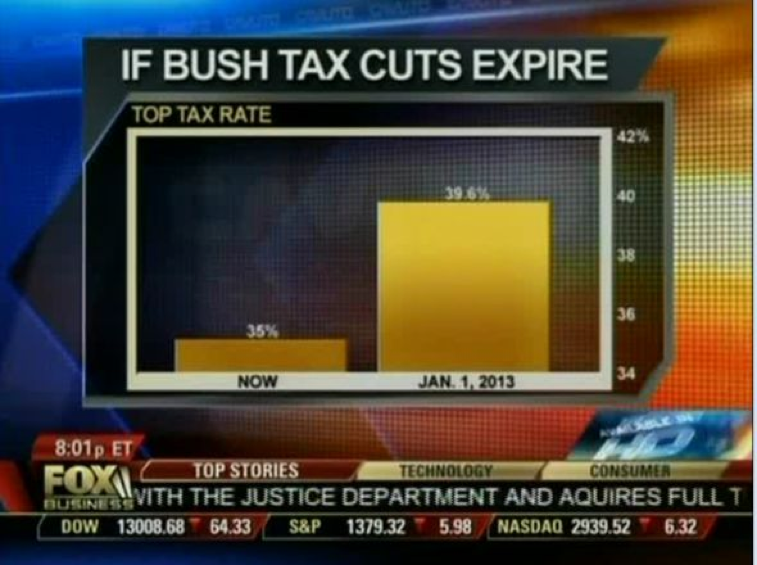
\includegraphics{1.png}
\caption{}
\end{figure}

Reference: How Writers Use Misleading Graphs To Manipulate You BY RYAN
MCCREADY, AUG 10, 2017
\url{https://venngage.com/blog/misleading-graphs/} Misleading graph,
wikipedia
\url{https://en.wikipedia.org/wiki/Misleading_graph\#Truncated_graph}

\chapter{Fundamentals}\label{fundamentals-1}

History Data visualization has comes a long way. Prior to the 17th
century, data visualization already exists. Though display in other
format such as maps, the content are much similar to today's
visualization, which mostly presented geologic, economic, and medical
data. Here is useful link:
\url{http://www.dashboardinsight.com/news/news-articles/the-history-of-data-visualization.aspx}

Current research: Deceptive visualizations Data visualization is a
powerful communication tool to support arguments with numbers in a way
that is accessible and engaging. More people than ever before are making
their own charts and infographics, which is presenting a unique problem.
Despite the availability of some great charting resources, we are
witnessing an influx of poorly-designed misleading or downright
deceptive data visualizations. Here are useful links:
\url{https://medium.com/@Infogram/study-asks-how-deceptive-are-deceptive-visualizations-8ff52fd81239}
\url{https://www.datapine.com/blog/misleading-data-visualization-examples/}

\bibliography{book.bib,packages.bib}


\end{document}
